\documentclass[a4paper, 11pt,oneside]{book}
\usepackage{import}
\usepackage[T1]{fontenc}
\usepackage{hyperref}
\usepackage[utf8]{inputenc}
\usepackage{tocloft}
\usepackage[english,italian]{babel} 
\usepackage{graphicx} 
\usepackage[top=3cm,bottom=3cm,left=3cm,right=3cm,headheight=14pt]{geometry}
\usepackage{titlesec}
\usepackage{mathptmx}
\usepackage{fancyhdr}
\usepackage{float}
\usepackage{xcolor}
\usepackage{amsmath}
\usepackage{enumitem}
\usepackage[most]{tcolorbox}
\usepackage{caption}
\usepackage{subcaption}
\usepackage{array}
\usepackage{listing}

% metainformazioni
\title{Configuratore di auto}
\author{Moretto Mattia}


% personalizzazioni
\newtcolorbox{mybox}[2][]{
    title = #2,#1,breakable,
    colback = black!0!white, 
    colframe = black, 
    halign title = flush center,
    fontupper = \itshape,
    fontlower = \itshape,
    segmentation style={solid, black!100}
}

\graphicspath{{immagini/}}
\newcommand{\add}[1]{\import{componenti/}{#1}}
\newcommand{\spacing}{\par\bigskip\noindent}

% \titleformat{\chapter}{\bf\huge\scshape}{\thechapter}{1em}{}

\hypersetup{
    colorlinks = false,
    linkbordercolor = black,
    pdfborderstyle = {/S/U/W 1}
}

\definecolor{backcolor}{rgb}{0.95,0.95,0.92}
\definecolor{codegreen}{rgb}{0,0.6,0}

\lstdefinestyle{MyStyle}{
    backgroundcolor=\color{backcolor},   
    commentstyle=\color{codegreen},
    keywordstyle=\color{magenta},
    basicstyle=\ttfamily\footnotesize,
    breakatwhitespace=false,         
    breaklines=true,                 
    keepspaces=true,                 
    numbers=left,       
    numbersep=5pt,                  
    showspaces=false,                
    showstringspaces=false,
    showtabs=false,                  
    tabsize=2,
}

\lstset{style=MyStyle}

\pagestyle{fancy}
% fine personalizzazioni


%Inizio Elaborato
\begin{document}


% input file frontespizio.tex
\add{frontespizio}

% Indice
\begingroup
    \hypersetup{hidelinks}
    \tableofcontents
    \addtocontents{toc}{~\hfill\textbf{Pagina}\par}
\endgroup

\begingroup
    \hypersetup{hidelinks}
    \listoffigures
\endgroup


% Primo capitolo
\chapter{Desiderata}
    \'E richiesto lo sviluppo di un sistema informatico per la vendita online di automobili di un gruppo multi-concessionaria con la possibilità di configurare la versione
    di automobile desiderata.\\
    Il gruppo vende auto di diversi modelli, raggruppati per marca. Per ogni modello di auto il sistema deve poter memorizzare:
    \begin{itemize}
        \item Un nome univoco
        \item Una descrizione
        \item Le dimensioni (altezza, lunghezza, larghezza, peso e volume del bagaglio)
        \item Possibili immagini che permettano di vedere l'auto da vari punti di vista con (potenzialmente diversi colori)
    \end{itemize}
    Il sistema dovrà registrare tutte le ruote a catalogo e definire possibili optional:
    \begin{itemize}
        \item Il colore
        \item Possibili aggiunte
        \begin{itemize}
            \item Ruotino di scorta
            \item Ruota di scorta
            \item Vetro oscurato
            \item Interni in pelle
            \item Ruote con diametri maggiori di quello standard
        \end{itemize}
    \end{itemize}
    Per ogni optional deve essere definito il prezzo e se applicabile o meno al modello scelto.\\
    Per alcuni modelli deve poter essere applicato uno sconto che può variare da un mese all'altro e viene applicato in fase di costruzione del preventivo ed opportunamente 
    indicato. Il cliente deve anche indicare, in caso di acquisto, dove intende ritirare l'auto.
    \spacing
    Un generico utente anche senza autenticarsi deve poter configurare l'auto per la quale pensa di chiedere un preventivo. Successivamente nel momento in cui decide di richiedere
    un preventivo al gruppo è richiesto che l'utente si registri (nel caso in cui non lo fosse già) e poi effetturare l'accesso al sistema. Solo a seguito di ciò avrà quindi la
    possibilità di richiedere la valutazione della sua auto usata allegando delle fotografie.
    \spacing
    Nel caso di valutazione dell'usato, il preventivo verrà finallizato da una persona del negozio, che provvederà a valutare l'usato. Il preventivo potrà essere prodotto anche come file pdf:
    \spacing
    Il sistema memorizza i preventivi effettuati. Entro 20 giorni il potenziale acquirente può confermare il preventivo e pagare un acconto, per ordinare l'auto nella configurazione
    indicata. Il sistema provvederà a proporre una data di consegna (a un mese più 10 giorni per ogni optional richiesto) entro la quale avere l'auto ordinata.
    \spacing
    Il gruppo ha diversi sedi in Italia dov'è possibile ritirare l'auto ordinata. Per ogni sede il sistema deve memorizzare nome, indirizzo completo e tutti gli ordini relativi a quella sede.
    \spacing
    Il sistema deve permettere agli impiegati del gruppo di accedere tramite autenticazione al sistema e gestire i preventivi che richiedono la valutazione dell'usato. Gli impiegati potranno poi 
    gestire gli ordini e avvisare i clienti quando l'auto ordinata è pronta per la consegna (dopo il pagamento dell'iporto dovuto).
    \spacing
    La segreteria amministrativa del gruppo è responsabile dell'inserimento delle informazini su modelli e optional di ogni marca. Essa può accedere al sistema e visualizzare i preventivi per cliente, per marca
    e per negozio di consegna richiesto.
    \spacing
    Il sistema deve inoltre permettere all'utente di configurare l'auto avendo un controllo del prezzo finale dell'auto ad ogni momento. 



% Secondo capitolo
\chapter{Specifiche Tecniche}
    \section{Tecnologie utilizzate}
        Di seguito vengono elencate e descritte le principali tecnologie utilizzate per lo sviluppo del software per dare un idea generale di come è composto quanto richiesto. Queste particolari scelte progettuali sono dettate dalla confidenza
        e praticità nell'utilizzo da parte dei componenti del gruppo nell'utilizzarli anche in ambito lavorativo.
        \subsection{C++}
            Si tratta di un linguaggio di programmazione di alto livello orientato agli oggetti e fortemente tipizzato, è stato sviluppato come estensione del linguaggio C ed introdotto negli anni 80.
            C++ combina le caratteristiche della programmazione procedurale con quelle della programmazione orientata agli oggetti, permattendo la creazione di software più complessi, efficienti e modulari.
            \'E ampiamente utilizzato nello sviluppo di sistemi operativi, applicazioni desktop, giochi, software per dispositivi embedded e applicazioni ad alte prestazioni. Grazie alla sua flessibilità e potenza, C++ rimane
            uno dei linguaggi più influenti e utilizzati nel mondo della programmazione.
        \subsection{Angular}
            Angular è un framework open-source per lo sviluppo di applicazioni web, mantenuto da Google e basato su TypeScript, Angular facilita la creazione di applicazioni web dinamiche e reattive grazie alla sua architettura
            a componenti, che consente la suddivisione del codice in moduli riutilizzabili e facilmente gestibili. Tra le sue caratteristiche principali, Angular offre strumenti per il data binding, la gestione delle forme, l'iniezione
            di dipendenze e il routing, semplificando lo sviluppo di applicazioni complesse e scalabili. Grazie alla sua versalità e potenza Angular è una scelta popolare per la creazione di applicazioni web moderne, sia in ambito 
            enterprise che consumer.
        \subsection{Json}
            JSON (JavaScript Object Notation) è un formato leggero per lo scambio di dati, facile da leggere e scrivere sia per le persone che per le macchine. Utilizzato principalmente per trasmettere dati tra un server e un client web, JSON
            rappresenta le informazioni in un formato testuale strutturato basato su coppia chiave-valore, simile ad un oggetto JavaScript. Grazie alla sua semplicità e compatibilità con la maggior parte dei linguaggi di programmazione, JSON è
            diventato uno standard ampiamente adottato per l'interscambio di dati nelle applicazioni web e nelle API. Nel nostro progetto è stato utilizzato come database.
        \subsection{Pistache}
            Pistache è un framework leggero e open-source scritto in C++ per lo sviluppo di server HTTP. Progettato per essere semplice ed efficiente, Pistache offre un architettura basata su eventi e supporta la creazione di server web ad alte prestazioni,
            in grado di gestire numerose connessioni simultanee. \'E particolarmente adatto per lo sviluppo di API RESTfull, grazie alla sua capacità di gestire richieste e risposte HTTP in modo intuitivo e veloce. Pistache è una scelta popolare per gli sviluppatori 
            in C++ che cercano un framework minimalista ma potente per costruire applicazioni web scalabili e performanti.
        \subsection{Postman}
            Si tratta di uno strumento collaborativo per lo sviluppo e il test delle API. Consente agli sviluppatori di inviare richieste HTTP, visualizzare le risposte e automatizzare i test semplificando il processo di interazione con le API durante lo sviluppo.
            Con Postaman è possibile creare e gestire raccolte di richieste, configurare ambienti, variabili e documentare le API in modo efficiente. Grazie alla sua interfaccia user-friendly e alle potenti funzionalità di automazione è diventato uno strumento essenziale 
            per lo sviluppo, debug e la gestione della API migliorando così la produttività e la collaborazione nei team di sviluppo
        \subsection{Karma}
            Karma è un test runner per Javascript sviluppato come parte dell'ecosistema Angular. Progettato per facilitare il processo di testing, consente di eseguire test unitari e di integrazione direttamente nel browser, garantendo che il codice funzioni correttamente
            in diversi ambienti. Supporta vari framework di test come Jasmine e Mocha e si integra facilmente nei flussi di lavoro e i sviluppo continuo. Con Karma,gli sviluppatori, possono automatizzare l'esecuzione dei test su più browser e dispositivi ricevendo feedback immediato
            sulle modifiche al codice, il che rende il processo di sviluppo delle applicazioni Angular più affidabile e efficiente
        \subsection{Jasmine}
            Jasmine è un framework di testing per Javascript, ampiamente utilizzato nel contesto Angular per scrivere test unitari.E'basato su un'architettura di testing behavior-driven(BDD), che consente di secrivere il comportamento del codice in modo leggibile e intuitivo. Jasmine 
            non richiede dipendenze esterne e offre un ampia gamma di funzionalità, come gli assertion, gli spy per il monitoraggio delle funzioni e la gestione asincrona del test. Quando integrato con angular, Jasmine permette di testare i singoli componenti, servizi e moduli assicurandosi
            che ogni parte dell'applicazione funzioni come previsto contribuendo con alla creazione di codice affidabile a manutenibile
    \section{Formule applicate}
        Nello sviluppo di questo software ci siamo soffermati su due punti in particolare che richiedevano precise formule per soddisfare la desiderata.
        La prima riguarda la fase di configurazione dell'auto dove il prezzo finale deve sempre essere controllabile in ogni momento pertanto il calcolo che viene fatto è il seguente:
        \begin{gather*}
            p_{f} = p_{0} + {\sum_{0}^{i}} p_{i} \\
            p_{f} = Prezzo \; finale \quad p_{0} = Prezzo \; base \\
            i = Numero \; componenti \; scelti \quad p_{i} = Prezzo \; componente
        \end{gather*}
        Viene omesso il fatto che al prezzo finale ottenuto può essere applicato uno sconto in quanto avverrebbe soltanto in fase di creazione del preventivo e dipende fortemente dal modello e dal periodo dell'ordine
        \spacing
        La seconda invece riguarda la data di consegna entro la quale l'utente puà ritirare l'auto ordinata che deve soddisfare il seguente presupposto:
        \begin{gather*}
            d_{c} > date(now)+(30 + i*10) \\
            d_{c} = data \; consegna \quad i = numero \; componenti
        \end{gather*}
    

            
        

% Terzo capitolo
\chapter{Casi d'uso}
    I casi d'uso permettono di modellare i requisiti funzionali ossia quei requisiti che specificano cosa deve essere fatto. Essi sono indipendenti dalla tecnologia,
    dall'architettura, dalla piattaforma e dal linguaggio di programmazione.\\
    I casi d'uso specificano cosa ci si aspetta da un sistema e allo stesso tempo nascondono come il sistema lo implementa. Sono una sequenza di azioni che producono un risultato osservabile da un attore e vengono utilizzati
    per descrivere i requisiti iniziali (analisi) e a convalidare l'architettura.\\
    Un ottimo elemento per rappresentarli è il diagramma dei casi d'uso che procediamo quindi a sviluppare.
    \section{Diagramma dei casi d'uso}
        Si tratta di un diagramma che esprime un comportamento desiderato o offerto e, solitamente, l'oggetto esaminato è un sistema o una sua parte. Permette di individuare chi o che cosa ha a che fare con il sistema (attore) e cosa
        esso può fare.\\
        Tipicamente il diagramma dei casi d'uso è la prima cosa ad essere creata in un processo o ciclo di sviluppo nell'ambito dell'analisi dei requisiti
        \spacing
        Per comporre correttamente il diagramma dobbiamo prima fare un passo indietro e individuare tutti i casi d'uso che compongono il sistema.
        \spacing
        Per sviluppare i casi d'uso è necessario prima analizzare quella che è la desiderata, ossia, in questo caso, la consegna fornita per lo sviluppo del progetto che è stata riportata nel \hyperlink{chapter.1}{capitolo 1}. Formalizzare i desiderata
        individuando i requisiti è un elemento fondamentale in quanto una specifica errata o incompleta è una delle cause principali del fallimento dei progetti software.
        \spacing
        Procedendo quindi per step andiamo ad analizzare tutto quello che ci viene richiesto, che possiamo riassumere nel seguente modo:
        \begin{itemize}
            \item Software per la vendita di auto (configurabili) online
            \item Un catalogo che prevede diversi modelli raggruppati per marca e con i relativi optional e immagini illustrative
            \item Sconti sui sigoli modelli applicabili e opportunamente indicati in fase di crazione del preventivo
            \item La possibilità per gli utenti che utilizzano la piattaforma di configurare in ogni momento l'auto per cui pensano di richiedere un preventivo anche senza autenticarsi e, previa autenticazione, la possibilità
            di richiedere il preventivo e la valutazione del suo usato
        \end{itemize}
        Lo step successivo è quindi quello di individuare gli attori ossia ruoli che vengono assunti dagli utenti o altre entità che interagiscono col sistema. Un attore deve essere per forza esterno al sistema inoltre non necessariamente deve essere un
        umano. Nello sviluppo del nostro progetto gli attori individuati sono i seguenti:
        \begin{itemize}
            \item Utente/Cliente
            \item Impiegati
            \item Segreteria
        \end{itemize}
        Per ognuno di questi attori è ora possibile individuare i casi d'uso ossia l'obiettivo prefissato all'inzio del capitolo e sono gli elementi che  permettono la creazione del diagramma
        \begin{itemize}
            \item Il cliente consulta il catalogo, si registra e può effettuare acquisti
            \item Il cliente personalizza l'auto
            \item Il cliente richiede un preventivo e sceglie la sede per il ritiro
            \item l cliente può richiedere la valutazione dell'usato
            \item Gli impiegati si autenticano e gestiscono i preventivi che richiedono la valutazione dell'usato
            \item Gli impiegati  gestiscono gli ordini e avvisano quando l'auto è pronta per la consegna
            \item La segreteria si occupa dell'inserimento delle informazioni dei modelli e optional per ogni marca
            \item La segreteria può visualizzare ogni preventivo per cliente, marca e per negozio di consegna
            \item Il cliente paga l'acconto
            \item Il cliente ritira l'auto
        \end{itemize}
        \spacing
        Arrivati a questo punto ci è possibile procedere allo sviluppo del diagramma del caso d'uso collegando innanzitutto i diversi attori ai relativi casi d'uso attraverso le associazioni ossia il primo elemento di collegamento.\\
        Successivamente ci siamo occupati delle diverse dipendenze tra i casi d'uso, nel nostro caso abbiamo deciso di utilizzare:
        \begin{itemize}
            \item \textbf{Include:} dipendenza dove il caso incluso fa parte del comportamento di quello che lo include, si tratta di un comportamento obbligatorio
            \item \textbf{extend:} dipendenza dove il caso d'uso che estende specifica un incremento di comportamento a quello esteso, si tratta di un comportamento opzionale che gestisce casi particolari
        \end{itemize}
        Una volta esserci soffermati su tutti i punti siamo arrivati a creare il diagramma nella sua interezza che si presenta nel seguente modo:
        \begin{figure}[H]
            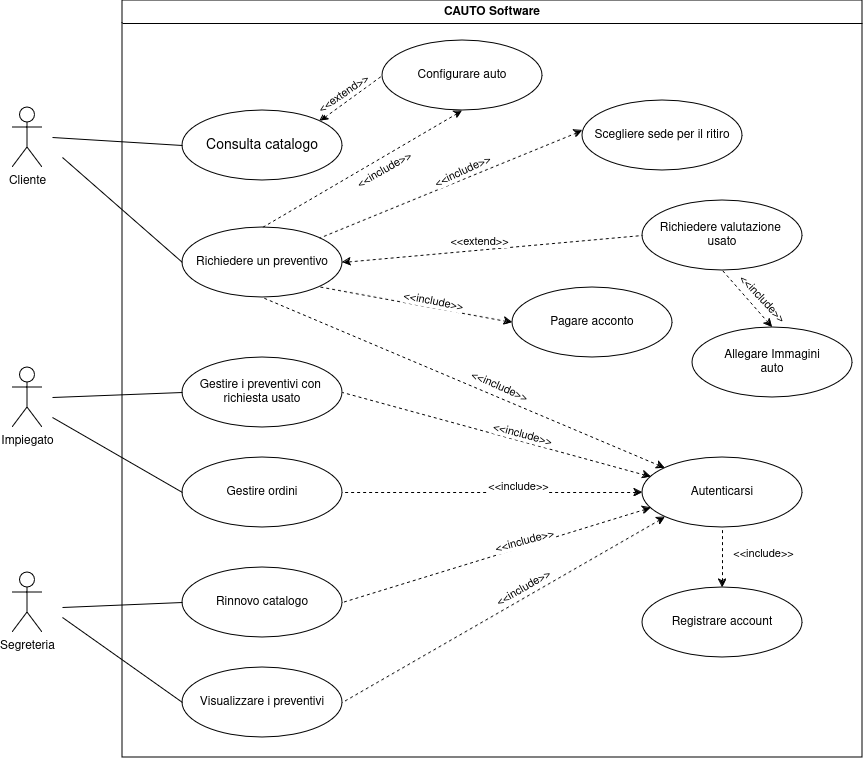
\includegraphics[width=\textwidth]{Diagramma_casi_d'uso.png}
            \caption{Diagramma Casi d'uso}
            \label{fig:diagramma_casi_d'uso}
        \end{figure}
        \spacing
        Quanto riportato è il diagramma d'uso inteso come punto di partenza per lo sviluppo del progetto. Si ha però l'esigenza di abbinare a questo
        diagramma delle specifiche testuali, più formali, in quanto non sono adatti a mostrare la sequenza temporale delle operazioni oppure lo stato del
        sistema e degli attori prima e dopo l'esecuzione. \'E necessario quindi procedere con la descrizione (specifica) dei casi d'uso
    \section{Schede di specifica}
        Ogni caso d'uso ha un nome e una specifica, quest'ultima è composta da:
        \begin{itemize}
            \item \textbf{precondizioni:} condizioni che devono essere vere prima che il caso d'uso di possa eseguire
            \item \textbf{sequenza degli eventi:} i passi che compongono il caso d'uso.
            \item \textbf{postcondizioni:} condizioni che devono essere vere quando il caso d'uso termina l'esecuzione
        \end{itemize}
        Partendo quindi dagli utenti/clienti si procede ad analizzare quelle che sono le schede di specifica che lo riguardano
        \begin{mybox}{Consulta catalogo}
           \textbf{ID:} CU1
           \tcbline
           \textbf{Attori}: Utente
           \tcbline
           \textbf{Precondizioni:} Nessuna
           \tcbline
           \textbf{Sequenza}: 
           \begin{enumerate}
            \item Entrare nella pagina dedicata al catalogo delle auto
            \item Osservare e configurare auto
           \end{enumerate}
           \tcbline
           \textbf{Postcondizioni}: Nessuna
        \end{mybox}
        \spacing
        \'E importante evidenziare il fatto che dal consultare il catalogo non è stata specificata alcuna postcondizione in quanto per come il software è stato
        predisposto un utente generico ha la possibilità di consultarlo senza alcun vincolo. Il caso d'uso appena analizzato lo si può quindi definire un'azione "base"
        prevista dal software.\\
        Si passa quindi ad analizzare il successivo caso d'uso che lo si può considerare quello principale all'interno di quello che è il funzionamento dell'applicazione.
        \begin{mybox}{Richiedere un preventivo}
            \textbf{ID:} CU2
            \tcbline
            \textbf{Attori}: Utente
            \tcbline
            \textbf{Precondizioni:} Essersi Registrato sulla piattaforma
            \tcbline
            \textbf{Sequenza}: 
            \begin{enumerate}
                \item Effettuare l'accesso alla piattaforma
                \item Configurare l'auto che ha intenzione di acquistare
                \item
                \begin{enumerate}
                    \item Richiedere direttamente preventivo
                    \item Richiedere la valutazione del proprio usato 
                \end{enumerate}
                \item Scegliere la sede per effettuare il ritiro dell'auto
                \item Attendere finalizzazione del preventivo
                \item Entro 20 giorni confermare il preventivo
            \end{enumerate}
            \tcbline
            \textbf{Postcondizioni}: Pagare acconto
        \end{mybox}
        \spacing
        Elaborate le schede di specifica legate agli utenti si procede ad analizzare quelle relative agli impiegati
        \begin{mybox}{Gestire i preventivi con richiesta usato}
            \textbf{ID:} CU3
            \tcbline
            \textbf{Attori}: Impiegato
            \tcbline
            \textbf{Precondizioni:} \begin{enumerate}
                \item Un cliente ha richiesto la valutazione dell'auto usata durante la richiesta di un preventivo
                \item Essere registrato alla piattaforma
                \tcbline
            \end{enumerate} 
            \textbf{Sequenza}: 
            \begin{enumerate}
                \item Effettuare l'accesso alla piattaforma
                \item Accedere alla pagina dedicata con la lista dei preventivi da finalizzare
                \item Procedere a valutare l'usato
            \end{enumerate}
            \tcbline
            \textbf{Postcondizioni}: Finalizzare il preventivo
        \end{mybox}
        \spacing
        \begin{mybox}{Gestire ordini}
            \textbf{ID:} CU4
            \tcbline
            \textbf{Attori}: Impiegato
            \tcbline
            \textbf{Precondizioni:} 
                \begin{enumerate}
                    \item Essere registrato alla piattaforma
                    \item Acconto del preventivo pagato dall'utente
                    \item Terminato tempo attesa per la data di consegna
                \end{enumerate} 
            \tcbline
            \textbf{Sequenza}: 
                \begin{enumerate}
                    \item Effettuare l'accesso alla piattaforma
                    \item Accedere alla pagina dedicata con la lista dei preventivi
                    \item Procedere ad avvisare l'utente che l'auto è pronta
                \end{enumerate}
            \tcbline
            \textbf{Postcondizioni}: Consegna l'auto nella sede indicata
        \end{mybox}
        \spacing
        Terminate le schede di specifiche che riguardano gli impiegati si procede con quelle legate alla segreteria
        \begin{mybox}{Rinnovo catalogo}
            \textbf{ID:} CU5
            \tcbline
            \textbf{Attori}: Segreteria
            \tcbline
            \textbf{Precondizioni:} Essere registrato alla piattaforma
            \tcbline
            \textbf{Sequenza}: 
                \begin{enumerate}
                    \item Effettuare l'accesso alla piattaforma
                    \item Accedere alla pagina dedicata con il catalogo delle auto
                    \item Inserimento di informazioni su modelli e optional di ogni marca
                \end{enumerate}
            \tcbline
            \textbf{Postcondizioni}: Nessuna
        \end{mybox}
        \spacing
        Il caso d'uso che riguarda il rinnovo del catalogo è un'azione fine a se stessa, nel senso che si tratta di qualcosa che viene svolto
        dalla segreteria come parte del proprio lavoro, da questa azione non ne consegue nessun'altra ma è importante per avere il catalogo sempre
        aggiornato e influisce sui casi d'uso degli altri attori. Lo stesso vale per la prossima scheda, si potrebbe definire la segreteria come un attore passivo.
        \begin{mybox}{Visualizzare i preventivi}
            \textbf{ID:} CU6
            \tcbline
            \textbf{Attori}: Segreteria
            \tcbline
            \textbf{Precondizioni:} Essere registrato alla piattaforma
            \tcbline
            \textbf{Sequenza}: 
                \begin{enumerate}
                    \item Effettuare l'accesso alla piattaforma
                    \item Accedere alla pagina dedicata con la lista dei preventivi
                    \item Visualizzare i preventivi per cliente, marca e negozio di consegna richiesto
                \end{enumerate}
            \tcbline
            \textbf{Postcondizioni}: Nessuna
        \end{mybox}



%quarto capitolo
\chapter{Diagramma della classi}
    Un diagramma delle classi è un tipo di diagramma utilizzato nella modellazione ad oggetti. Serve per rappresentare la struttura statica di un sistema mostrando le classi, gli attributi, i metodi
    e le relazioni tra di esse come l'ereditarietà, l'associazione e la composizione. Si tratta di uno strumento fondamentale per la progettazione del software poichè consente di visualizzare e definire
    chiaramente l'architettura del sistema, facilitando la comprensione, la manutenzione e l'implementazione del codice.
    \spacing
    Si tratta del secondo step che abbiamo deciso di sviluppare in quanto serviva a dare un'idea generale della struttura del processo e permettere una stesura iniziale del codice in base alla metodologia che abbiamo deciso di adottare descritta nel capitolo dedicato. 
    All'interno del diagramma ogni classe viene rappresentata in forma di un rettangolo, che può avere fino a 3 slot:
    \begin{itemize}
        \item nome e l'eventuale stereotipo (in UpperCamelCase, obbligatorio)
        \item attributi (in lowerCamelCase, opzionali)
        \item operazioni (in lowerCamelCase, opzionali)
    \end{itemize}
    Ogni classe a sua volta si divide in:
    \begin{itemize}
        \item \textbf{classi di analisi:} solitamente contengono solo quelli più importanti e spesso specificano solo il nome
        \item \textbf{classi di progettazione:} forniscono una specifica completa (implementabile) della classe e dei suoi attributi
    \end{itemize}
    Per rappresentare invece le istanze delle classi si utilizza una notazione molto simile, quinid avranno anch'esse una forma rettangolare. Le differenze sostanziali stanno:
    \begin{itemize}
        \item Il titolo degli oggetti è sottolineato e nella forma "nome:classe" con nome opzionale
        \item Non hanno uno slot per le operazioni, possono invece definire valori per gli attributi
    \end{itemize}
    Fatta questa premessa si procede a mostrare mostrare il diagramma delle classi nella sua interezza e successivamente verrà fornita una breve descrizione di come è stato composto.
    \begin{figure}[H]
        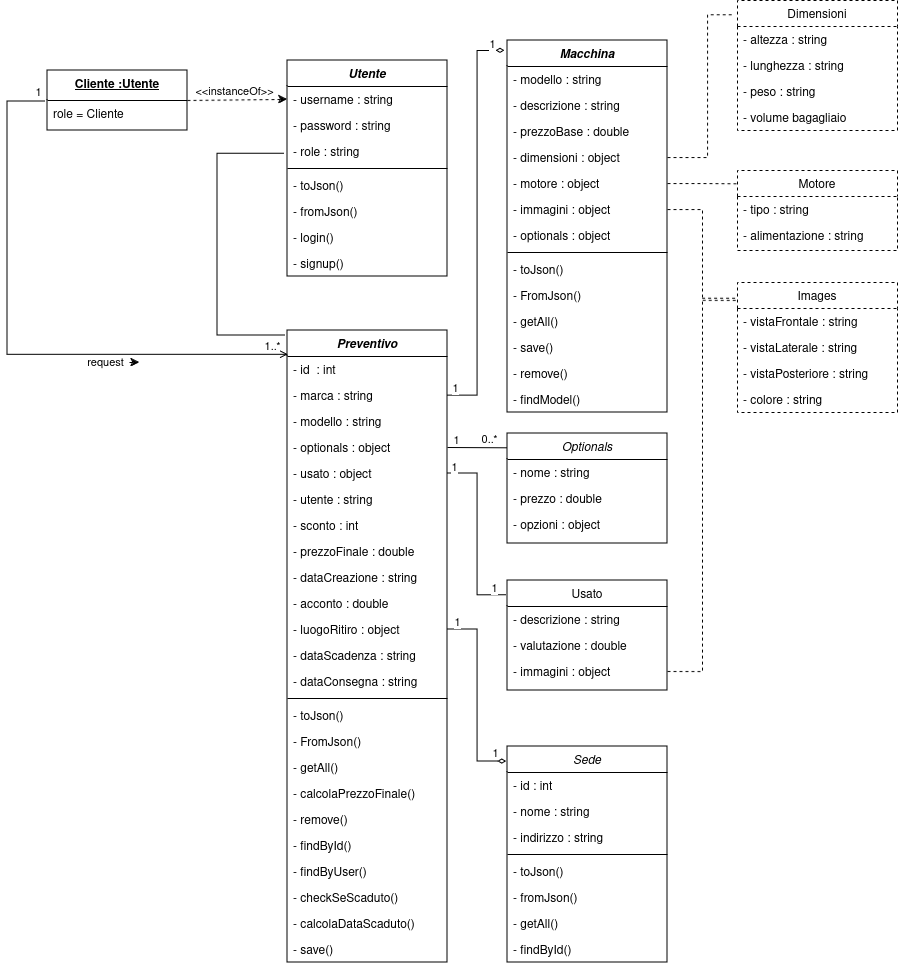
\includegraphics[width=\textwidth]{diagramma_delle_classi.png}
        \caption{Diagramma delle Classi}
        \label{fig:diagramma_delle_classi}
    \end{figure}
    \spacing
    All'interno del diagramma sono state riportate tutte le classi inserite all'interno del codice. Per completezza abbiamo deciso di mostrare anche tutte le operazioni e gli attributi che abbiamo creato, inoltre per scelte progettuali le abbiamo rese tutte
    pubblico, come si può vedere dal simbolo riportato accanto al nome\\
    Per quanto riguarda invece i tipi di collegamento abbiamo scelto di utilizzare:
    \begin{itemize}
        \item \textbf{<<instanceOf>>:} \'Abbiamo deciso di rappresentare una istanza per la classe utente, dove si va a passare l'attributo "role". questo
              è stato pensato per indicare la registrazione sulla piattaforma da parte dell'utente. A differenza degli altri due non ha possibilità di scegliere, il ruolo deve essere sempre definito
        \item \textbf{Associazione:} si tratta di un tipo di relazione generico che va ad indicare l'esistenza di un collegamento tra le istanze delle classi
        \item \textbf{Realizzazione:} identificabile dai riquadri che contengono <<interface>> e si tratta di una relazione semantica in cui il fornitore presenta una specifica e il cliente la realizzano
        \item \textbf{Dipendenza:} si tratta di una forma più debole di relazione tra classi e operazioni
        \item \textbf{Aggregazione:} si tratta di una relazione poco forte dove le due parti possono esistere anche da sole ed inoltre ognuna di esse può appartenere a più aggregazioni
    \end{itemize}
    \spacing
    Dall'immagine si possono vedere dei riquadri leggermente diversi che non sono propriamente elementi del diagramma delle classi per questo motivo abbiamo deciso di rappresentarli solamente con linee tratteggiate.
    Questa scelta è stata fatta in quanto alcune classi sono state composte con degli object e per poter dare chiarezza su come è veramente composta la classe. Quindi i blocchi in questione sono da intendere come un espansione
    dell'elemento object di riferimento che mostra gli attributi di cui è composto


% quinto capitolo
\chapter{Diagrammi d'interazione}
    Si tratta di diagrammi di comportamento che modellano le interazioni tra varie entità di un sistema inoltre permettono di visualizzare
    lo scambio di messaggi trà entità nel tempo. Il loro scopo principale è quello di mostrare come un certo comportamento viene realizzato dalla collaborazione
    delle entità in gioco.\\
    Sostanzialmente permette di illustrare il comportamento del sistema da una prospettiva interna inoltre possono avere diversi livelli di astrazione.\\
    Per comporre un diagramma di interazione sono necessarie due cose:
    \begin{itemize}
        \item Un comportamento da realizzare tratto da un classificatore di contesto come per esempio:
        \begin{itemize}
            \item Un caso d'uso
            \item im'operazione di classe
        \end{itemize}
        \item Una serie di elementi che realizzano il comportamento come:
        \begin{itemize}
            \item attori
            \item istanze di classe
        \end{itemize}
    \end{itemize}
    Generalmente nei diagrammi di interazione non compaiono direttamente classificatori come le classi, al loro posto ci sono:
    \begin{itemize}
        \item \textbf{Istanze} di classificatori (oggetti, istanze di attori)
            \begin{itemize}
                \item rappresenta uno specifico oggetto, e solo quello.
            \end{itemize}
        \item \textbf{Linee di vita} (lifeline) di classificatori
            \begin{itemize}
                \item è più generale.
                \item rappresenta un'istanza arbitraria di un classificatore.
                \item fornisce modi per specificare come quest'istanza viene scelta
                \item esprime il ruolo giocato da un'istanza senza preoccuparsi della sua identità
            \end{itemize}
    \end{itemize}
    La differenza tra questi due elementi è sottile ma, in generale, è preferibile usare le linee di vita
    \spacing
    In tutto ci sono 4 tipi di diagrammi di interazione ma andremo ad elaborare solamente il \textbf{diagramma di sequenza} che, come dice il nome, è adatto a mostrare la sequenza
    temporale degli avvenimenti per ogni entità nel diagramma e cominciamo sviluppando quelli relativi ai casi d'uso presi singolarmente
    \spacing
    \section{Casi d'uso}
        Per quanto riguarda i casi d'uso del Cliente viene omessa la consulta del catalogo in quanto l'iterazione con il sistema è veramente minima se non quasi nulla pertanto anche rappresentandola tramite
        diagramma non mostrerebbe molte più informazioni rispetto a quelli precedentemente trattati. Si procede quindi a mostrare quello riguardante la creazione del preventivo
        \begin{figure}[H]
            \centering
            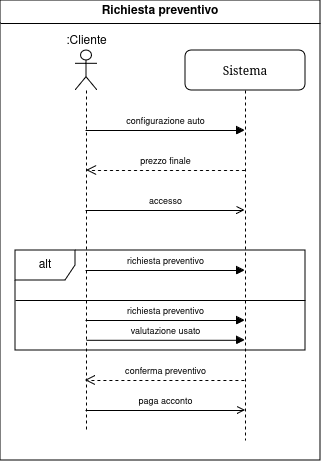
\includegraphics[scale=0.75]{sequence_diagram_preventivo.png}
            \caption{Diagramma di sequenza Cliente}
            \label{fig:diagramma_sequenza_utente}
        \end{figure}
        \spacing
        A livello temporale si è cercato di esprimere in sequenza come dovrebbe avvenire il processo per la richiesta di un preventivo da parte di un cliente.
        Innanzitutto l'utente può consultare liberamente ogni auto a catalogo e ha la facoltà di configurarla, durante questo processo il sistema dovrà fornire in ogni momento
        il prezzo finale dell'auto. Una volta scelta e configurata l'auto il cliente può procedere con l'acquisto ma prima di poter fare ciò deve essere per forza autenticato.
        Da qui in avanti avrà dunque la possibilità di procedere in due strade, la prima è quella di richiedere direttamente il preventivo, nella seconda invece può scegliere anche di richiedere 
        la valutazione del proprio usato. Per entrambi i casi l'ultimo passaggio che rimane da fare è quello di attendere di ricevere conferma da parte del sistema dopo la quale l'utente può procedere a pagare
        l'acconto dovuto ed attendere che l'auto sia pronta per poterla andare a ritirare nella sede da lui specificata.
        \spacing
        Si procede dunque a mostrare il diagramma creato per gli Impiegati.
        \begin{figure}[H]
            \centering
            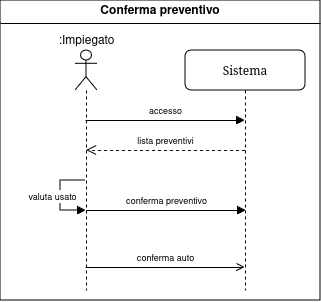
\includegraphics[scale=0.75]{sequence_diagram_confirm.png}
            \caption{Diagramma di sequenza Impiegato}
            \label{fig:diagramma_sequenza_impiegato}
        \end{figure}
        \spacing
        In questo caso il passaggio che avviene è più semplice, una volta che l'impiegato effettua l'accesso alla piattaforma, quest'ultima fornirà la lista di tutti
        i preventivi che sono in attesa di conferma ossia quei preventivi nel quale è stata richiesta la valutazione dell'usato. Quello che deve fare l'impiegato è quindi controllare le immagini che sono state fornite
        e stimare un prezzo per l'auto usata, dopodichè può procedere con la conferma del preventivo. Una volta fatto questo non gli resta altro che avvisare il cliente quando l'auto è pronta per il ritiro
        \spacing
        Procediamo infine a mostrare il diagramma creato per la segreteria.
        \begin{figure}[H]
            \centering
            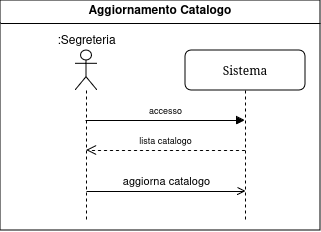
\includegraphics[scale=0.75]{sequence_diagram_catalog.png}
            \caption{Diagramma di sequenza Segreteria}
            \label{fig:diagramma_sequenza_segreteria}
        \end{figure}
        \spacing
        Anche in questo caso la procedura è molto semplice, la segreteria effettua l'accesso alla piattaforma che provvederà a fornire la lista di tutte le auto a catalogo. Avrà quindi la possibilità di aggiornare le auto
        già presenti oppure aggiungere nuove auto.
    \section{Sistema}
        \begin{figure}[H]
            \centering
            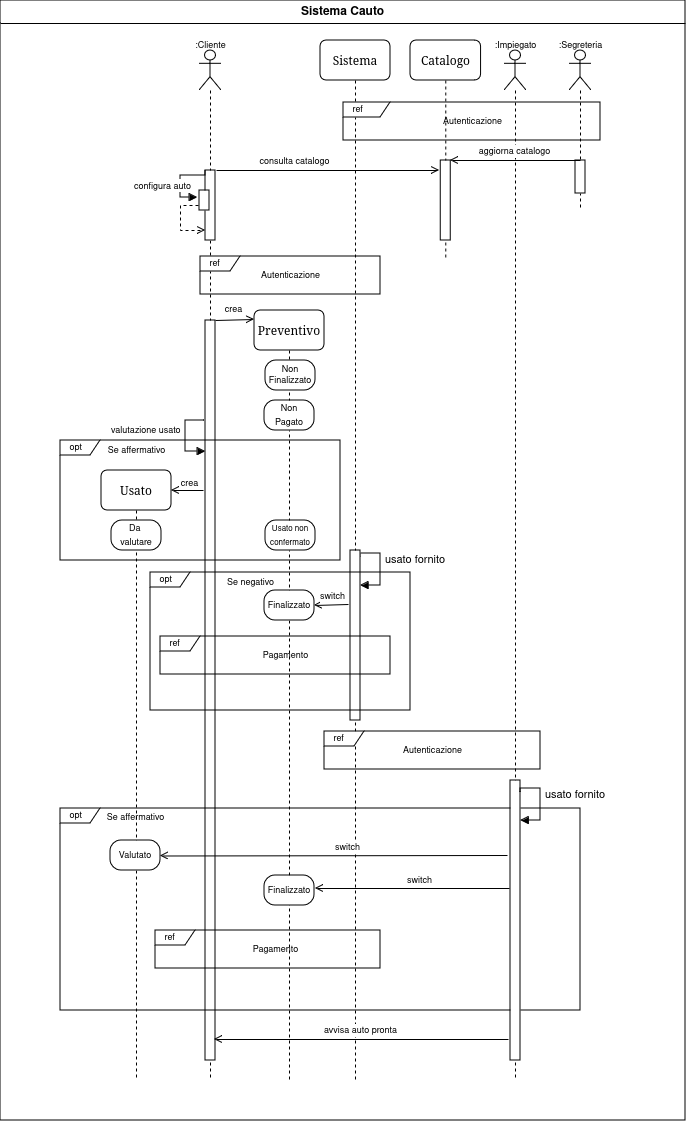
\includegraphics[scale=0.5]{sequence_diagram_sistema.png}
            \caption{Diagramma di sequenza sistema}
            \label{fig:diagramma_sequenza_sistema}
        \end{figure}
        \spacing
        Quanto riportato è il diagramma di sequenza che rappresenta il funzionamento dell'intero sistema a livello temporale di quello che accadrebbe dall'inizio alla fine nello svolgimento della sua funzione principale,
        mentre di seguito vengono riportati i diagrammi che fanno riferimento all'operatore ref utilizzato nell'immagine soprastante.
        \begin{figure}[H]
            \centering
            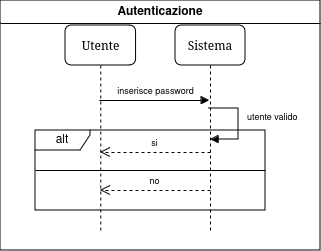
\includegraphics[scale=0.75]{sequence_diagram_rif_autenticazione.png}
            \caption{Diagramma di sequenza autenticazione}
            \label{fig:diagramma_sequenza_autenticazione}
        \end{figure}
        \begin{figure}[H]
            \centering
            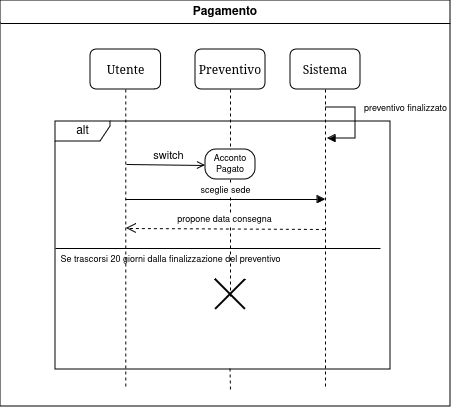
\includegraphics[scale=0.75]{sequence_diagram_rif_pagamento.png}
            \caption{Diagramma di sequenza pagamento}
            \label{fig:diagramma_sequenza_pagamento}
        \end{figure}
        \spacing
        \newpage\noindent
        Con il diagramma riportato nella figura 5.4 abbiamo messo in evidenza come le varie entità collaborino nel fornire l'output richiesto dalla desiderata
        \spacing
        Nella costruzione di tutti i diagrammi di attività riportati abbiamo utilizzato:
        \begin{itemize}
            \item \textbf{Messaggi:}
            \begin{itemize}
                \item chiamata sincrona: ossia quei messaggi che bloccano chi li manda in attesa di un messaggio di ritorno del destinatario
                \item chiamata asincrona: dove il mittente non si aspetta una risposta e prosegue immediatamente
                \item chiamata di ritorno: anche se opzionali abbiamo scelto di utilizzarli ogni qual volta è stata definita una richiesta sincrona per indicare
                cosa ci si aspetta per poter proseguire
                \item creazione: come dice il nome duranta la sequenza servono ad indicarela creazione di un nuovo oggetto
                \item distruzione: similmente a quello di creazione indica la distruzione dell'oggetto, una volta arrivati a quel punto non sarà più accessibile
            \end{itemize}
            \item \textbf{Attivazioni annidate:} le linee vita mandano messaggi a se stesse si tratta di operazioni frequenti per indicare per esempio invocazioni di operazioni private
            \item \textbf{stato:} è definito come una condizione o situazione durante la vita dell'oggetto in cui esso soddisfa una condizione, uno stato o aspetta un evento
            \item \textbf{operatori:} determina la semantica dell'esecuzione di un frammento combinato ossia una sottoarea che racchiude una parte dell'interazione e le modalità della sua esecuzine, quelli utilizzati sono:
            \begin{itemize}
                \item opt: corrisponde a if/then e accetta solo un operando che viene eseguito se e solo se la guardia è valutata true
                \item alt: corrisponde a case/select e accetta un qualunque numero di operandi e ne esegue al più uno
                \item ref: rende i diagrammi di sequenza modulari, l'operatore contiene il nome di un'altra interazione che viene eseguita qui
            \end{itemize}
        \end{itemize}


% sesto capitolo
\chapter{Diagrammi di Stato e attività}
    Si tratta di diagrammi che permettono di descrivere il comportamento, procediamo ad analizzarli singolarmente
    \section{Diagramma di stato}
        Serve a modellare il comportamento (generalmente di una sola entità) come variazione del suo stato interno. Come dice il nome esso permette di descrivere la sequenza di stati in cui si trova un oggetto durante il suo
        ciclo di vita e in risposta agli eventi.\\
        In UML qualunque oggetto può essere associato a una macchina a stati che descrive il funzionamento delle sue istanze ed è caratterizzato da 3 elementi:
        \begin{itemize}
            \item Uno \textbf{stato}, ossia una condizione o situazione nella vita di un oggetto in cui esso:
            \begin{itemize}
                \item soddisfa una condizione
                \item esegue un'attività
                \item aspetta un evento
            \end{itemize}
            \item Un \textbf{evento}, ossia la specifica di un'occorrenza che ha una collocazione nel tempo e nello spazio
            \item Una \textbf{transizione}, ossia il passaggio da uno stato a un altro in risposta ad un evento. Oltre allo stato d'origine e destinazione una transizione può specificare
            \begin{itemize}
                \item \textbf{event:} un trigger che attiva il passaggio di stato
                \item \textbf{guard:} una condizione che, se vera, permette il passaggio di stato
                \item \textbf{action:} un'azione che risulta dal cambio di stato
            \end{itemize}
        \end{itemize}
        Procediamo quindi ad elaborare i due diagrammi di stato che abbiamo deciso di sviluppare
        \begin{figure}[H]
            \centering
            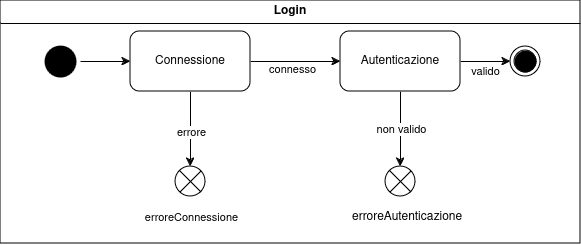
\includegraphics[scale=0.55]{diagramma di stato_autenticazione.png}
            \caption{Diagramma di stato autenticazione}
            \label{fig:diagramma_stati_autenticazione}
        \end{figure}
        \begin{figure}[H]
            \centering
            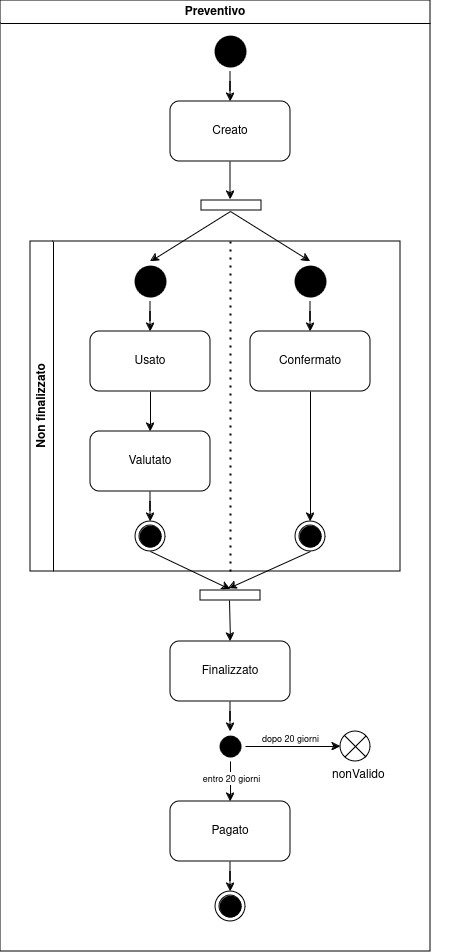
\includegraphics[scale=0.49]{diagramma di stato_preventivo.png}
            \caption{Diagramma di stato preventivo}
            \label{fig:diagramma_stato_preventivo}
        \end{figure}
        \pagebreak\noindent
        Nella costruzione del diagramma sono stati utilizzati solamente gli elementi base, l'unico elemento particolare che è stato aggiunto per il preventivo
        è lo \textbf{stato composito e sincronizzazione} che permette di suddividere la complessità del modello. Dall'esterno si vede un macro-stato al cui interno però ci sono altri stati. Con la sincronizzazione invece si divide lo stato composito in sotto-diagrammi
        e si utilizzano gli operatori fork e join.
    \section{Diagramma di attività}
        I diagrammi di attività servono per modellare un attività relativa ad un qualsiasi oggetto,tra i suoi usi più comuni troviamo il modellare il flusso di un caso d'uso, modellare il funzionamento di un operatore di classe e modellare un algoritmo e sono composti da tre elementi 
        principali:
        \begin{itemize}
            \item Nodi \textbf{azione:} specificano unità di comportamento e possono invocare un'attività, un comportamento o un'operazione
            \item Nodi \textbf{oggetto:} specificano oggetti usati come input e output di azioni
            \item Nodi \textbf{controllo:} specificano il flusso delle attività.
        \end{itemize}
        Per capire la semantica dei diagrammi di attività bisogna immaginare delle entità chiamate token, che viaggiano lungo il diagramma. Il flusso di questi token definisce quello dell'attività inoltre essi possono rimanere fermi in un nodo azione/oggetto in attesa che si avveri una condizione su una freccia,
        oppure una precondizione o postcondizione su un nodo. Un nodo azione viene eseguito quando sono presenti token su tutti gli archi in entrata e tutte le precondizioni sono soddisfatte. Quando invece termina un azione vengono generati control token su tutti gli archi in uscita.
        \spacing
        Procediamo a mostrare il suddetto diagramma:
        \begin{figure}[H]
            \centering
            \includegraphics[trim={0 36cm 0 0},clip, scale=0.6]{diagramma di attività.png}
            \phantomcaption
        \end{figure}
        \begin{figure}[H]
            \continuedfloat
            \centering
            \includegraphics[trim={0 0 0 18cm},clip, scale=0.6]{diagramma di attività.png}
            \caption{Diagramma di attività}
            \label{fig:diagramma_attività}
        \end{figure}
        \spacing
        Oltre a quanto già riportato, nella creazione del diagramma sopra riportato abbiamo utilizzato dei particolari nodi di controlli ossia:
        \begin{itemize}
            \item \textbf{nodi iniziali/finali:} classici nodi del diagramma, il disco nero marca l'inizio dell'attività e quindi la generazione del token mentre quello nero bordato indica che l'attività ha termine
            \item \textbf{nodi di decisione:} hanno un input e vari output mutuamente esclusivi
            \item \textbf{nodi fork:} hanno un ingresso e varie uscite, ciò corrisponde al token in ingresso che viene duplicato verso tutte le uscite
            \item \textbf{nodi join:} hanno vari ingressi e una sola uscita, quando sono presenti token su tutti gli ingressi, viene prodotto almeno un token in uscita
            \item \textbf{nodi finali di flusso} quando raggiunti da un token, causano la terminazione solo del flusso che li ha toccati
        \end{itemize}
        \spacing
        Arrivati alla conclusione del capito si può notare come i diagrammi di stato e di attività siano in pratica la stessa cosa semplicemente usati in modo diversi. Sostanzialmente i diagrammi di attività sono diagrammi di stato in cui gli stati vengono convertiti in azioni.
        Infatti come si può notare, confrontando quanto riportato si può notare una certa similitudine nella struttura e negli elementi tra i vari diagrammi



% settimo capitolo
\chapter{Test del Software}
    Per verificate la solidità, l'efficenza, la chiarezza e la precisione nel soddisfare la richiesta del software prodotto sono state eseguite le seguenti attività:
    \begin{enumerate}
        \item Revisione della desiderata e del documento creato
        \item Verifica della consistenza tra diagrammi e codice prodotto
        \item Ispezione del codice per verificare la corretta struttura e ricerca errori a livello di leggibilità
        \item Unit test eseguito con l'ausilio di Karma e Jasmine per il Front End e Postman per il Back End
        \item Test da parte degli sviluppatori del software
        \item Test da parte di un utente esterno con raccolta feedback
    \end{enumerate}
    L'esecuzione di questi test ha portato a modifiche, migliorie e nuove implementazioni del software che a conti fatti corrisponderebbe a diverse versione di una beta prima del rilascio/vendita effettiva del software che possono essere riassunti nel seguente modo
    \begin{center}
        \begin{tabular}{|| m{0.1\textwidth} | m{0.8\textwidth} ||}
            \hline
            Versione & Descrizione \\
            \hline
            \hline
            v0.1 & Si tratta di una versione base durante la creazione del documento per portarsi avanti con lo sviluppo dove erano presenti semplici elementi comuni a tutte le interfaccie\\
            \hline
            v0.2 & Si tratta della versione prodotta una volta concluso il documento e quindi tutta la parte di analisi e progettazione \\
            \hline
            v0.3 & Si tratta della versione pordotta dovo aver terminato i diversi Unit Test \\
            \hline
            v0.4 & Si tratta della versione prodotta dopo aver concluso i test da parte degli sviluppatori \\
            \hline
            v1.0 & Si può considerare la prima release del software dovo aver eseguito i test da parte degli utenti esterni. Si tratta delle versione del software presentata oggi \\
            \hline
        \end{tabular}
    \end{center}
    \section{Revisione e Ispezione}
        In questa fase siamo semplicemente partiti analizzando nuovamente la desiderata per accertarci che non ci fosse sfuggito niente durante le prime letture e analisi del contenuto. Una volta accertati che avessimo inquadrato tutti i punti siamo passati a controllare il documento
        confrontando i diversi diagrammi UML prodotti con il codice sviluppato per verificarne la consistenza. Si è trattato del punto più decisivo nello sviluppo del software.\\
        Una volta conclusa l'attività siamo passati a ricontrollare il codice per controllare che non fossero presenti errori a livello di leggibilità e struttura del software, dopo aver eseguito questo passaggio si può considerare il software quasi completo, i restanti test che abbiamo fatto
        hanno solamento portato a correzzioni o piccole rivisatazioni
    \section{Unit Test}
        Per la parte di unit test, tramite gli strumenti descritti nel Capitolo 2, abbiamo testato il corretto funzionamento delle implementazioni del Software sviluppato. Partendo dal file main.cpp riportato qui sotto abbiamo provato ad effettuare delle prove per la creazione, rimozione e modifica di tutti gli elementi
        necessari sulla piattaforma.
        \spacing
        \lstinputlisting[label={lst:listing-cpp}, language=C++]{file/main.cpp}
        \spacing
        I test effettuati hanno utilizzato delle chiamate API che a loro volta erano state precedentemente testate tramite PostMan, i test sono stati eseguiti per ogni singola chiamata API creata. Di seguito riportiamo un esempio per quanto riguarda la creazione del preventivo, è comunque possibile vedere
        tutte le chiamate dall'apposita applicazione.
        \begin{figure}[H]
            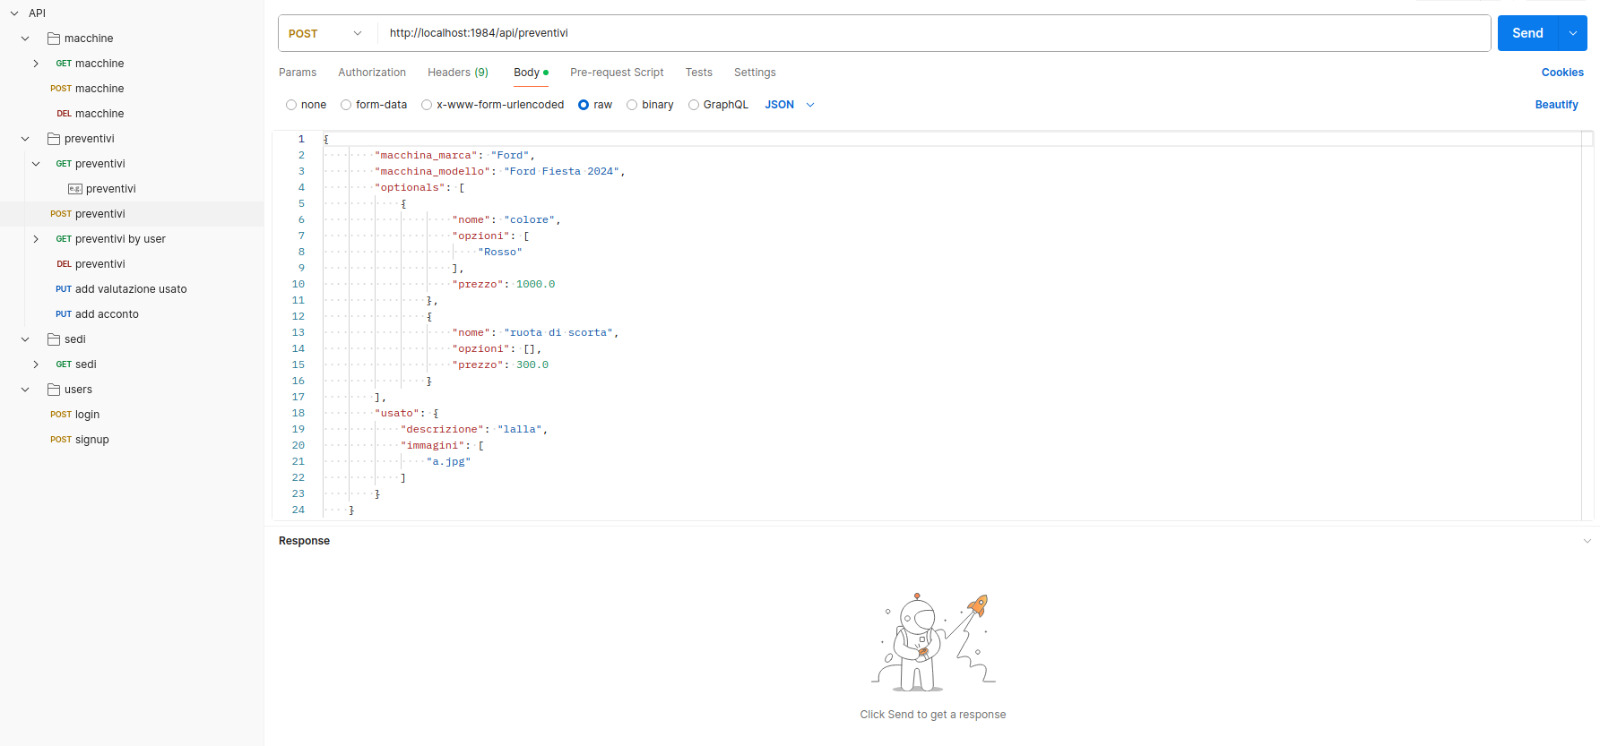
\includegraphics[width=\textwidth]{Postman_POST.jpeg}
            \caption{Postman POST}
            \label{fig:postman_post}
        \end{figure}
        \spacing
        Oltre ai test sopra riportati abbiamo applicato dei controlli anche sulla Vista utilizzando la suite di Angular (Karma e Jasmine già analizzati nell'apposita sezione) che si occupa di lanciare i test direttamente sul browser, verificando l'integrità dei singoli componenti e il collegamento tra
        i diversi modelli. Di seguito viene riportato un esempio di quello che viene restituito dall'interfaccia di test, nello specifico riguardante il servizio dedito ad importare i vari moduli per le chiamate http ed effettuare le chiamate alle api.
        \begin{figure}[H]
            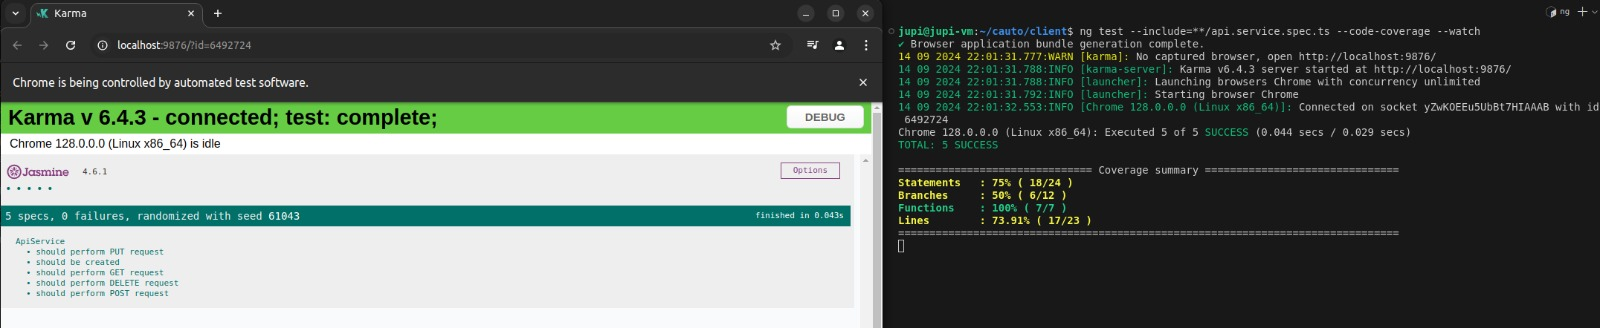
\includegraphics[width=\textwidth]{Karma_Test.jpeg}
            \caption{Test con Karma}
            \label{fig:Karma_test}
        \end{figure}
        \spacing
    \section{Test degli Sviluppatori}
        In questa fase abbiamo testato personalmente il sistema per controllare che le funzioni previste dal software funzionassero correttamente. Nello specifico i test che si sono svolti sono i seguenti:
        \begin{itemize}
            \item \textbf{Autenticazione:} Per questo test abbiamo provato a simulare l'accesso da partedi utenze relative al personale, ossia impiegato e segreteria, per controllare se funzionasse correttamente e restituisse la visualizzazione dedicata alle mansioni che devono svolgere. Per l’utenza dei clienti si è provato a creare l’utenza e poi l'accesso di un cliente già registrato
            \item \textbf{Catalogo:} Per questo test abbiamo provato ad accedere alla pagina dedicata al catalogo e abbiamo verificato che restituisse correttamente tutte le auto presenti
            \item \textbf{Preventivo:} La prima cosa che abbiamo controllato in questa fase è quella che la pagina dedicata per la creazione del preventivo fosse accessibile anche senza essere loggati, per permettere la configurazione della macchina. Una volta fatto questo abbiamo provato a creare un preventivo, abbiamo verificato l'effettivo salvataggio e che fosse correttamente mostrato nella pagina dedicata della lista dei preventivi per tutte le utenze interessate
            \item \textbf{Auto usata:} Durante la fase di creazione del preventivo è possibile aggiungere una descrizione e delle foto per la valutazione dell'usato. Abbiamo quindi valutato che l'inserivento venisse effettuato correttamente e che fosse reperibile nelle diverse pagine di visualizzazione dei preventivi
            \item \textbf{Impiegato:} rovando ad accedere con un utenza da impiegato abbiamo verificato che si vedessero correttamente tutti i preventivi sia quelli che richiedevano la valutazione dell’usato sia quelli già avvisati che erano in attesa della consegna. Abbiamo controllato che riuscisse a vedere correttamente le immagini per la valutazione e che riuscisse a completare la valutazione
            \item \textbf{Segreteria:} Provando ad accedere con un utenza da segreteria abbiamo verificato che vedesse correttamente tutte le pagina ossia la lista dei preventivi e del catalogo. Nella pagina dei preventivi abbiamo controllato che ci fossero tutti e che avesse la possibilità di filtrarli mentre
            nella pagina del catalogo abbiamo controllato che potesse modificare, aggiungere e rimuovere sia auto e preventivi
            \item \textbf{Acquisto:} Dopo tutte le premesse, con un preventivo finalizzato, abbiamo testato che il pagamento dell'acconto e la proposta della data di consegna funzionasse correttamente. Come ultimo test abbiamo inoltre verificato che passati i 20 giorni senza che avvenisse il pagamento il preventivo
            venga rimosso
        \end{itemize}
    \section{Test degli Utenti}
    Come test finale abbiamo fatto provare l'applicazione a diversi utenti con più o meno dimestichezza con la tecnologia. Per lo svolgimento del test è stata solamente fornita la finalità del software. Nella prima fase abbiamo dato agli utenti piena libertà di navigazione mentre in un secondo momento abbiamo richiesto
    alcune particolari simulazioni indicando cosa volevamo ottenere per testare in particolare le utenze degli impiegati e delle segreteria. Durante ogni fase del test abbiamo risposto ad eventuali domande e raccolti tutti i feedback ricevuti, in questo modo abbiamo avuto la possibilità di correggere alcuni piccoli 
    problemi e migliorato
    il software del punto di vista dell'usabilità.



% ottavo capitolo
\chapter{Pattern Architetturali}
    Un pattern architetturale è una soluzione collaudata e riutilizzabile per affrontare problemi comuni nella progettazione dell'architettura del software. Esso definisce una struttura organizzativa generale per un sistema fornendo linee guida su come suddividere il software in componenti, moduli e livelli e su come questi 
    interagiscono tra loro. Questa tipologia di pattern aiutano a garantire che il software sia scalabile, manutenibile e flessibile e la sua adozione consente ai progettisti di beneficiare delle esperienze accumulate nella risoluzione di problemi simili, migliorando l'efficienza e la qualità del progetto.
    \begin{figure}[H]
        \centering
        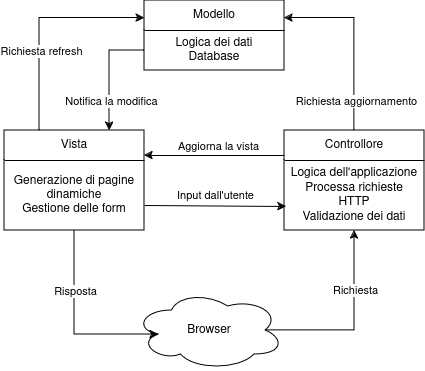
\includegraphics[scale=0.75]{Architettura MVC.png}
        \caption{Architettura MVC}
        \label{fig:architettura_mvc}
    \end{figure}
    \spacing
    Per il nostro progetto abbiamo scelto di utilizzare il \textbf{pattern MVC}. Come dice il nome, questo modello è caratterizzato da tre elementi:
    \begin{itemize}
        \item \textbf{Modello:} Rappresenta la logica di gestione dei dati. Esso gestisce i dati dell'applicazione, risponde alle richieste della View per l'accesso ai dati e risponde alle istruzioni del Controller per modificare i dati
        \item \textbf{Vista:} Si occupa della presentazione dei dati all'utente. Essa visualizza i dati che riceve dal Modello e riflette eventuali cambiamenti nei dati. E' responsabile dell'interfaccia utente e di come i dati vengono presentati all'utente finale
        \item \textbf{Controllore:} Funziona come intermediario tra il Modello e la Vista. Esso riceve l'input dell'utente attraverso la Vista, elabora tale input (eventualmente interagendo con il Modello) e aggiorna la Vista di conseguenza.
    \end{itemize}
    Le azioni dell'utente saranno catturate dai listener del controllore, quest'ultimi sono pensati per reagire di conseguenza andando a modificare le informazioni contenute nel Modello e di conseguenza aggiornetà la vista che rappresenta il Modello\\
    \'E stato scelto questo modello in quanto si adatta bene a quello che abbiamo progettato, i componenti dei modelli e del controllore possono essere riutilizzati con diverse viste il che aumenta l'efficenza nello sviluppo di nuove funzionalità o versioni dell'applicazione. Il modello MVC è una scelta popolare per lo sviluppo 
    di applicazioni web e software, soprattutto in contesti in cui la manutenibilità, la modularità e la collaborazione sono essenziali.
    \spacing
    

% nono capitolo
\chapter{Pattern adottati}
    I design pattern sono per l'appunto pattern che utilizzano metodi e classi di un linguaggio OO. Durante lo progettazione, la maggior parte dello sviluppo è avanzato attraverso la conoscenza dei programmatori dovuta all'esperienza lavorativa, non sono stati quindi stati seguiti consciamente dei particolari pattern. Alla fine dei conti 
    l'unico con il quale ci siamo allineati è il \textbf{Data Access Object Pattern} (DAO).\\
    Questo pattern nello specifico viene utilizzato per separare la logica di accesso ai dati dalla logica delle operazioni, in sostanza agisce come interfaccia tra il programma e la fonte di dati, come per esempio un database, consentendo di eseguire operazioni di CRUD (Create, Read, Update, Delete) senza esporre direttamente
    i dettagli di implementazione dei meccanismi di persistenza. Il DAO Pattern è strutturato nel seguente modo:
    \begin{itemize}
        \item \textbf{Interface}(astrazione del DAO): definisce i metodi per l'accesso ai dati come getUsr() e createUser()
        \item \textbf{Concrete DAO}: Implementa l'interfaccia e cotiene la logica specifica per interagire con il database o altre fonti di dati
        \item \textbf{Entity Model}: la classe che rappresenta l'entità che mappa i dati(ad esempio User) contenente gli attributi corrispondenti alle colonne del database
        \item \textbf{Service Layer}: Il livello che utilizza il DAO per accedere e gestire la logica del business
    \end{itemize}
    Questo particolare pattern è stato leggermente riaddatato secondo le nostre esigenze, infatti all'interno della nostra struttura non è presente l'interface in quanto abbiamo deciso di non creare alcuna classe astratta.
    Abbiamo deciso di utilizzarlo in linea generale nella costruzione delle API e comprende ottenimento, creazione, aggiornamento e rimozione di tutte le entità in gioco in questo progetto



% ottavo capitolo
\chapter{Note sul processo di sviluppo}
    Il progetto è stato sviluppato principalmente seguendo il modello di tipo a Cascata implementando alcuni aspetti del tipo Agile.
    Il modello a cascata è caratterizzato da fasi separate e distinte di specifiche e sviluppo, in linea di principio una fase deve essere completata prima di passare alla fase successiva. Il modello a cascata rende difficile "accogliere" i cambiamenti a processo avviato quindi non è l'ideale per rispondere ad eventuali modifiche
    richieste dal cliente. Al contrario però si presta molto bene nel caso in cui i requisiti siano ben chiari fin dall'inizio come per il nostro caso dove è stato proposto lo sviluppo di una desiderata che rimasta fissa. Il fatto dell'applicazione del modello a cascata è ben visibile anche dall'elaborato appena sviluppato. Ogni aspetto
    dello sviluppo è avvenuto passo per passo, abbiamo definito con chiarezza:
    \begin{itemize}
        \item I requisiti richiesti
        \item L'ideazione del design del software
        \item L'implementazione e gli Unit Test
        \item Test del sistema
    \end{itemize}
    Procedendo in questo modo abbiamo creato una solida base su cui lavorare nello step successivo riducendo così il rischio di "perdere tempo" nel dover tornare indietro  nell'accorgerci che qualcosa era stato definito in maniera errata. \\
    Per permettere comunque un lavoro più fluido si è deciso comunque di uscire un pò dalla rigida struttura del modello cascata per agevolare un pò le tempistiche visti gli impegni del gruppo. Periodicamente ci fornivamo a vicenda gli aggiornamenti riguardo ciò che avevamo
    fatto, in questo modo se uno doveva lavorare allo step successivo poteva cominciare a portarsi avanti con il lavoro defininendo almeno gli aspetti base e una volta terminato lo step antecedente poteva completarlo aggiungendo ciò che restava in sospeso.\\
    Per quanto riguardo l'intera implementazione ci siamo suddivisi i ruoli in base alla confidenza dei membri del gruppo sulle parti richieste da sviluppare, ciò ha permesso uno sviluppo più rapido in quanto abbiamo ridotto il rischio di problemi dovuti allo sviluppo simultaneo del codice. L'elemento chiave per la riuscita nello sviluppo del 
    software è stata la pianificazione dettagliata creata all'inizio che abbiamo seguito dall'inizio alla fine. Nell'ottica del team work eravamo comunque pronti a fornire supporto in caso di necessita sulle attività degli altri membri del gruppo.
    \section{Scelte Progettuali}
        Come già possibile intuire da quanto presentato il software è stato sviluppato con linguaggi diversi da quelli presentati al corso inoltre la struttura del codice non è composta da classi astratte, protette o private come quanto studiato dal linguaggio Java quest'anno. Tutto è stato creato come pubblico.\\
        Inoltre nonostante i vari test che abbiamo effettuato e le diverse release rilasciate siamo consapevoli che il software in fin dei conti è ancora in fase di sviluppo. Abbiamo implementato tutte le richieste derivanti dalla desiderata ma ci sono alcuni aspetti non presenti ad oggi alla presentazione per poterla definire completa. Ciò che manca viene inteso 
        come sviluppo futuro, e nello specifico si tratterebbe di:
        \begin{itemize}
            \item \textbf{Integration test:} Questo specifico test si riferisce al processo di verifica delle interfaccie tra due moduli software per verificare come i dati vengono trasferiti tra di loro, nel nostro caso andrebbe applicato per testare lo scambio tra la vista ed il controllore
            \item \textbf{Sicurezza e Crittografia:} In questo momento sul software non è stata implementata alcuna misura di sicurezza, essendo un qualcosa che deve essere pubblicata sul Web, al giorno d'oggi è di vitale importanza che vengano applicati degli accorgimenti per quanto riguarda la sicurezza. Prendiamo per esempio il login, in questo momento questi dati vengono
            passati da un modulo all'altro senza che vengano criptati, in questo stato chiunque sappia interciettare la chiamata può vedere tranquillamente i dati sensibili degli utenti, lo stesso vale per i possibili dati inseriti durante il pagamento
            \item \textbf{Sistemi di pagamenti:} Al momento della presentazione viene simulato l'inserimento del pagamento, però, per rendere il software veramente completo andrebbero implementati dei veri metodi di pagamento, almeno quelli classici come la carta di credito o PayPal.
            \item \textbf{Email per la conferma:} Si tratta di una possibile implementazione che ci è venuta in mente durante le fasi di revisione. Nella desiderata è stato fatto presente che l'impiegato si occupa anche di avvisare gli utenti nel momento in cui l'auto da lui ordinata è pronta per il ritiro, non è stato fatto però presente come avviene ciò. Ad oggi è stato deciso
            che si tratta di un qualcosa che avviene al di fuori del funzionamento del software per esempio tramite chiamata telefonica. Abbiamo ritenuto comunque interessante considerare il fatto di poter implementare una funzione che si occupa in automatico di avvisare un email all'utente utilizzando quella che ci ha fornito in fase di registrazione
        \end{itemize}
\end{document}